\section{Questionnaire}
To better understand the needs and goals of our audience, we conducted a questionnaire that reached out to 78 participants. Utilizing Google Forms, we efficiently gathered and analyzed responses to delve into the specifics of our application domain. The questionnaire was thoughtfully designed with carefully crafted questions divided into four main sections:

\begin{enumerate}
	\item \textbf{General Questions:}
	These questions aimed to gather broad insights into participants' backgrounds, demographics, and general preferences that could influence their interaction with our application.
	
	\item \textbf{Questions about the Application:}
	This section focused on probing participants' expectations, desires, and specific requirements related to our application. It aimed to uncover their motivations for potentially using our product and what features or functionalities they prioritize.
	
	\item \textbf{Personal Questions:}
	These questions delved into participants' individual experiences, challenges, and personal insights relevant to our application domain. This section aimed to capture nuanced feedback that could provide a deeper context for understanding their needs and preferences.
	
\end{enumerate}

By structuring our questionnaire in this manner and leveraging Google Forms for data collection and analysis, we aimed to gather comprehensive insights that will inform the development and refinement of our application. This approach ensures that we are aligning our product offerings closely with the expectations and requirements of our target audience, ultimately enhancing user satisfaction and engagement.\\
\clearpage
\subsection{General Questions}
\begin{figure}[htbp]
	\centering
	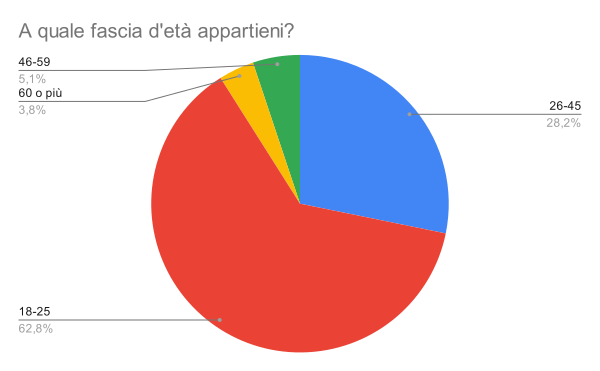
\includegraphics[width=0.8\textwidth]{../Draw.io diagrams/age_chart.png}  % Replace 'example-image' with the filename of your image
	\caption{The chart notice that the age groups of respondents coincides with our target age}
\end{figure}

\begin{figure}[htbp]
	\centering
	\includegraphics[width=0.8\textwidth]{../Draw.io diagrams/Qual è il tuo genere_.png}  % Replace 'example-image' with the filename of your image
	\caption{The chart notice the distribution of respondents between the gender.}
\end{figure}


\begin{figure}[htbp]
	\centering
	\includegraphics[width=0.8\textwidth]{../Draw.io diagrams/Il tuo paese di residenza è in Europa_.png}  % Replace 'example-image' with the filename of your image
	\caption{The chart shows that the location of respondents is in Europe that coincides with our target region.}
\end{figure}

\begin{figure}[htbp]
	\centering
	\includegraphics[width=0.8\textwidth]{../Draw.io diagrams/Attualmente lavori part-time o a tempo pieno in un paese della comunità europea_.png}  % Replace 'example-image' with the filename of your image
	\caption{The chart notice that the respondents with a job is greater than the respondents without a job, and this is another important index of our target profile.}
\end{figure}

\begin{figure}[htbp]
	\centering
	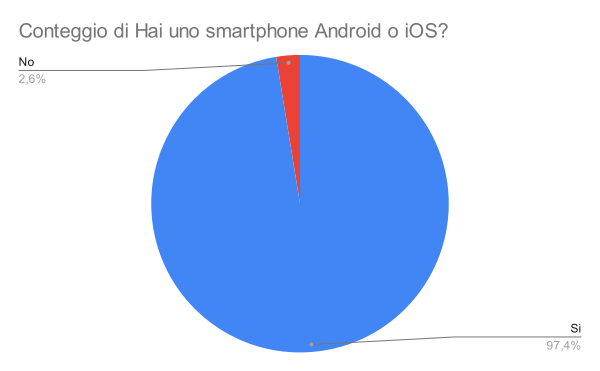
\includegraphics[width=0.8\textwidth]{../Draw.io diagrams/Conteggio di Hai uno smartphone Android o iOS_.png}  % Replace 'example-image' with the filename of your image
	\caption{The chart notice us that the totally of respondents have a smartphone with Android or iOS that is corresponding to our target technology.}
\end{figure}
\clearpage
\subsection{Application Questions}
\begin{figure}[htbp]
	\centering
	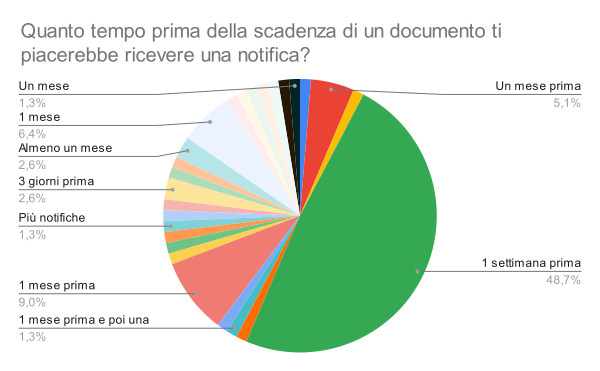
\includegraphics[width=0.8\textwidth]{../Draw.io diagrams/default_date.png}  % Replace 'example-image' with the filename of your image
	\caption{The chart shows the users preference about the default notification time.}
\end{figure}

\begin{figure}[htbp]
	\centering
	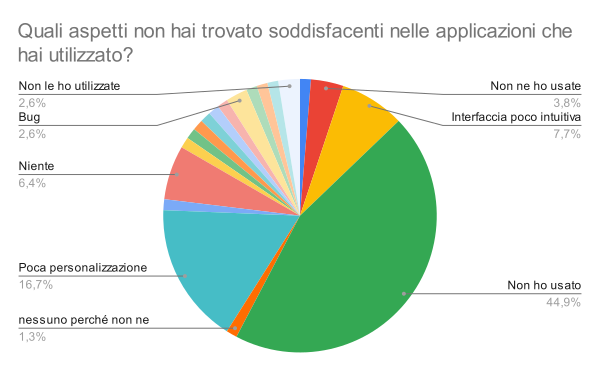
\includegraphics[width=0.8\textwidth]{../Draw.io diagrams/application_review.png}  % Replace 'example-image' with the filename of your image
	
	\caption{The chart shows what problems the users have found in the other applications.}
\end{figure}

\begin{figure}[H]
	\centering
	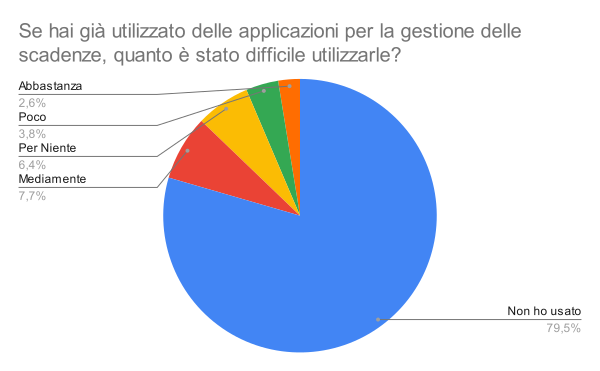
\includegraphics[width=0.8\textwidth]{../Draw.io diagrams/how_did_difficult_use_competitors.png}  % Replace 'example-image' with the filename of your image
	
	\caption{The chart shows how is difficult for the users use the other applications (competitors)}
\end{figure}
\clearpage
\subsection{Personal Questions}
\begin{figure}[htbp]
	\centering
	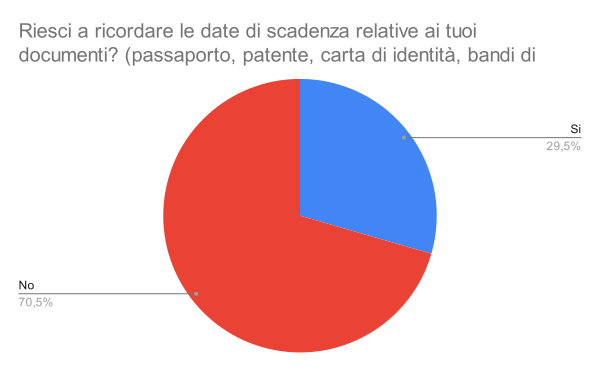
\includegraphics[width=0.8\textwidth]{../Draw.io diagrams/remember_dates.png}  % Replace 'example-image' with the filename of your image
	
	\caption{The chart shows how is difficult for the users remember the expiration dates}
\end{figure}
\begin{figure}[htbp]
	\centering
	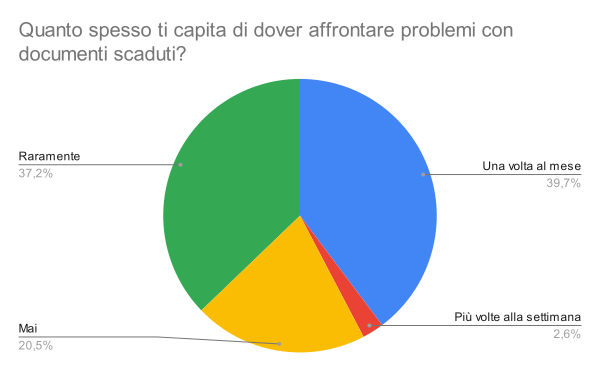
\includegraphics[width=0.8\textwidth]{../Draw.io diagrams/problems.png}  % Replace 'example-image' with the filename of your image
	
	\caption{The chart shows if the expiration date of a document was a problem for the real life}
\end{figure}
\begin{figure}[htbp]
	\centering
	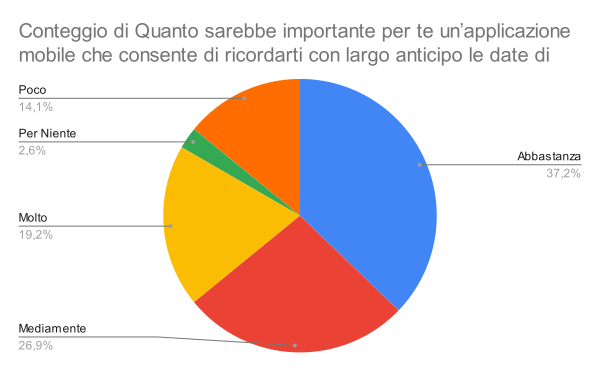
\includegraphics[width=0.8\textwidth]{../Draw.io diagrams/do_you_remember_expiration_dates.png}  % Replace 'example-image' with the filename of your image
	
	\caption{The chart shows how is important for the users using an helpfull application}
\end{figure}
\begin{figure}[htbp]
	\centering
	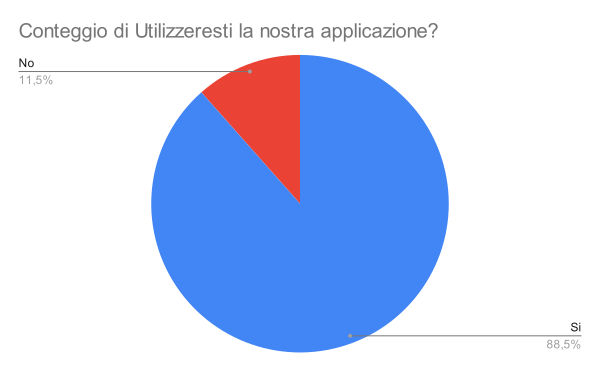
\includegraphics[width=0.8\textwidth]{../Draw.io diagrams/useresti_app.png}  % Replace 'example-image' with the filename of your image
	
	\caption{The chart shows if the users are available to use the our application}
\end{figure}